%\documentclass[CJKmath,a4paper,10pt]{exam-zh}
\documentclass[CJKmath,a4paper,10pt]{ctexart}
% 使用 exam-zh 官方参数设置页脚文字
%\examsetup{page={foot-content={物理习题第;页（共~;页）}}}
%\examsetup{page={foot-content={\textbf{数学}习题\ \itshape 第;/~;页}}}
\usepackage{geometry}
\geometry{inner=1.5cm,outer=1.5cm,top=2.45cm,bottom=1cm}
\usepackage[dvipsnames,svgnames,x11names,table]{xcolor}

\usepackage{amsmath,amssymb}
%\RequirePackage{unicode-math} % Math fonts in xetexorluatex
%\setmathfont{texgyrepagella-math.otf}
%\setmainfont{STIXTwoText}[
%	Path=./fonts/STIXTwoText/,
%  Extension = .otf,
%  UprightFont = STIXTwoMath-Regular,
%  BoldFont = STIXTwoText-SemiBold,
%  ItalicFont = STIXTwoText-Italic,
%  BoldItalicFont = STIXTwoText-BoldItalic,
%]
%\setmathfont{STIXTwoMath-Regular.otf}

\usepackage{tikz,calc}
\usetikzlibrary{calc,arrows.meta,arrows,shadows.blur,tikzmark,angles,quotes,tikzmark,positioning,shapes.geometric,intersections} % 角度、箭头库
\usepackage{tkz-euclide} 
% By default all math in TikZ nodes are set in inline mode. Change this to
% displaystyle so that we don't get small fractions.
\everymath{\displaystyle}

\usepackage[most]{tcolorbox}
\tcbuselibrary{breakable, skins,theorems}


\usepackage{xkeyval}
\makeatletter 
%\usepackage{amsmath,amssymb,amsthm}
\usepackage{xkeyval} 
\tcbset{
    common/.style={
      fontupper=\rmfamily,
      lower separated=true,
      coltitle=black,
      colback=gray!5,
      boxrule=0.1pt,
      fonttitle=\bfseries,
      enhanced,
      breakable,
      top=8pt,
      before skip=8pt,
      attach boxed title to top left={yshift=-0.05in,xshift=0.15in},
      boxed title style={
      	boxrule=0pt,
        colframe=black,
        arc=0pt,
        outer arc=0pt,
        drop fuzzy shadow
     	},
      separator sign={.},
      drop fuzzy shadow
     },
    litistyle/.style={
     	%例题风格
     	common,
     	colframe=gray,% 
     	colback=white,
     	colbacktitle=Gold,
     	sharp corners,rounded corners=southeast,
     	overlay unbroken and last={
     		\node[anchor=south east, outer sep=0pt] at (\linewidth-width,0){\textcolor{black!60}{$\blacksquare$}};
     	}
    },
% -----------------------------------------------------------------------------
% Explanation: BreakableBox@title key
% The following defines a pgfkeys/tcolorbox key named
%   "BreakableBox@title" which accepts 2 arguments (see 
%   "/.code n args={2}"). When the key is used like
%   "BreakableBox@title={<env>}{<optTitle>}" the code below is executed
%   with #1=<env> and #2=<optTitle>.
%
% Purpose:
% - If the second argument (#2) is empty, set the tcolorbox title to
%     \csname <env>name\endcsname~\thetcbcounter
%   which expands to the environment name (e.g. "liti" -> \litiname)
%   followed by the current counter value.
% - If the second argument is provided, append " (#2)" to the title.
%
% Notes:
% - This relies on \makeatletter being active so that keys with '@'
%   are allowed in control sequence names.
% - \ifblank is used to test whether #2 is empty; ensure the package
%   that provides \ifblank (for example, etoolbox or xparse) is loaded
%   earlier if necessary.
% - Example usage inside the code: \tcbset{title={...}} sets the
%   tcolorbox title key accordingly.
%
         BreakableBox@title/.code n args={2}
              {
                \ifblank{#2}
                  {\tcbset{title={\csname #1name\endcsname~\thetcbcounter}}}
                  {\tcbset{title={\csname #1name\endcsname~\thetcbcounter\ (#2)}}}
              },
}      
  % define an internal control sequence \newbreakablebox for fancy mode's newtheorem
  % #1 is the environment name, #2 is the prefix of label, #3 is the style
  % style: thmstyle, defstyle, prostyle
  % e.g. \newbreakablebox{theorem}{thm}{thmstyle}
  % will define two environments: numbered ``theorem'' and no-numbered ``theorem*''
  % WARNING FOR MULTILINGUAL: this cs will automatically find \theoremname's definition,
  % WARNING FOR MULTILINGUAL: it should be defined in language settings.
  \newcommand{\newbreakablebox}[3]{
    \ifcsundef{#1name}{%
      % define a default name if not defined before
      \tcbset{BreakableBox@title/.code n args={2}{\tcbset{title={use newcommand define #1name}}} }
    }{\relax}
    \DeclareTColorBox[auto counter]{#1}{ g o t\label g }{
        common, % use common style
        #3, % use the style passed in
        IfValueTF={##1}
          {BreakableBox@title={#1}{##1}}
          {
            IfValueTF={##2}
            {BreakableBox@title={#1}{##2}}
            {BreakableBox@title={#1}{}}
          },
        IfValueT={##4}
          {
            IfBooleanTF={##3}
              {label={##4}}
              {VIVID@label={#2}{##4}}
          }
      }
    \DeclareTColorBox{#1*}{ g o }{
        common,#3,
        IfValueTF={##1}
          {BreakableBox@title={#1}{##1}}
          {
            IfValueTF={##2}
            {BreakableBox@title={#1}{##2}}
            {BreakableBox@title={#1}{}}
          },
      }
  }
% define several environment 
% we define headers like \definitionname before
\newcommand{\litiname}{例}
\newbreakablebox{liti}{def}{litistyle}
  
  
%补充内容
%%设置新字体
%%定义带圈数字命令
\newfontfamily{\nmfont}{circlenumber}
[%
Extension=.otf,
Path=./fonts/]

\newcommand{\quan}[1]{{\nmfont \symbol{#1}}}
\newcommand{\kk}[1]{\quan{\numexpr32+#1}}%\kk{<参数范围1-95>}96、97、98、99分别用\quan{196} \quan{197} \quan{199} \quan{201}

%脚注使用带圈数字
\newcommand*\kkctr[1]{%
  \protect\kk{\number\numexpr\value{#1}\relax}}
\renewcommand*\thefootnote{\textcolor{black}{\kkctr{footnote}}}

%%无悬挂脚注格式
\renewcommand\@makefntext[1]{%
  \setlength\parindent{2\ccwd}\selectfont
  \@thefnmark\ #1}

%修改\part，使其不分页
\def\@endpart{%
	\thispagestyle{empty}
  \vskip40\p@%
   \@afterheading}



\RequirePackage{enumitem}
%\newenvironment{myenum}{\begin{enumerate}[label=\protect\kk{\arabic*}]\small}{\end{enumerate}}%
\setlist{noitemsep}
\setlist[enumerate, 1]{label=\protect\kk{\arabic*},itemsep=0.5ex}  
\makeatother



%%%marker环境
\newtcolorbox{marker}[1][]{enhanced,before skip=2mm,
	after skip=3mm,fontupper=\rmfamily,
	boxrule=0.4pt,left=5mm,right=2mm,top=1mm,bottom=1mm,
	colback=yellow!50,colframe=yellow!20!black,
	sharp corners,rounded corners=southeast,
	arc is angular,arc=3mm,underlay={%
		\path[fill=tcbcolback!80!black] ([yshift=3mm]interior.south east)--++(-0.4,-0.1)--++(0.1,-0.2);
		\path[draw=tcbcolframe,shorten <=-0.05mm,shorten >=-0.05mm] ([yshift=3mm]interior.south east)--++(-0.4,-0.1)--++(0.1,-0.2);
		\path[fill=yellow!50!black,draw=none] (interior.south west) rectangle node[white]{\Huge\bfseries !} ([xshift=4mm]interior.north west);
	},
	drop fuzzy shadow,#1
}


\usepackage{graphicx}
\usepackage{float}



\begin{document}

\section{三点共线结合爪型模型}
\begin{liti}{}	
	\begin{minipage}{0.5\linewidth}
		$如图，在\triangle ABC中，M是BC的中点，点N在AC上，\\且AN=2NC,AM与BN相交于点P。\\求AP:PM 与 PB:PN的值$。
	\end{minipage}
	\begin{minipage}{0.45\linewidth}
		\begin{center}
			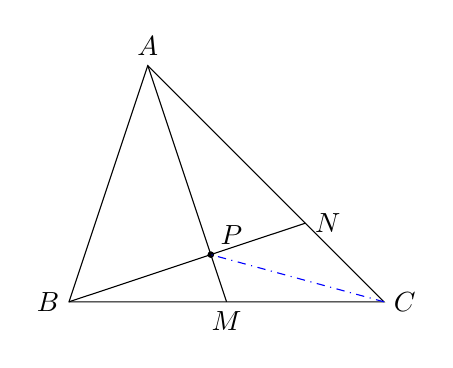
\begin{tikzpicture}[scale=1]
				\coordinate (A) at (1,3);
				\coordinate (B) at (0,0);
				\coordinate (C) at (4,0);
				\coordinate (M) at ($(B)!0.5!(C)$);
				\coordinate (N) at ($(A)!0.667!(C)$);
				% 绘制三角形边框
				\draw (A) -- (B) -- (C) -- cycle;
        % 绘制AM、BN并求交点P
        \path[name path=AM] (A) -- (M);
        \path[name path=BN] (B) -- (N);
        \path[name intersections={of=AM and BN, by=P}];
        \draw (A) -- (M) node[below] at (M) {$M$};
        \draw (B) -- (N) node[right]{$N$};
        \fill (P) circle (1.2pt) node[above right] {$P$};
				% 标注顶点
				\node[above]at (A) {$A$};
				\node[left] at (B) {$B$};
				\node[right] at (C) {$C$};
				%连接CP
				\draw[dash dot,blue] (C)--(P);
			\end{tikzpicture}
			%		\captionof{figure}{三角形 \(ABC\) 示例}
		\end{center}
	\end{minipage}
	%

	\tcblower
	如图所示，连接$CP$（关键步骤），则：
	\begin{align*}
	%&由\overrightarrow{CP}=\lambda\overrightarrow{CB}+\mu\overrightarrow{CA}\Rightarrow \overrightarrow{CP}=2\lambda\overrightarrow{CM}+\mu\overrightarrow{CA}。\because A,P,M三点共线，\therefore 2\lambda+\mu=1\\
	%&由\overrightarrow{CP}=\lambda\overrightarrow{CB}+\mu\overrightarrow{CA}\Rightarrow \overrightarrow{CP}=\lambda\overrightarrow{CB}+3\mu\overrightarrow{CN}。\because B,P,N三点共线，\therefore \lambda+3\mu=1
	&\because BPN三点共线，\therefore \overrightarrow{CP}=x\overrightarrow{CB}+(1-x)\overrightarrow{CN}\quad（三点共线，系数和为1）\\
	&\because APM三点共线，\therefore \overrightarrow{CP}=y\overrightarrow{CA}+(1-y)\overrightarrow{CM}\quad（同理）
	\end{align*}
	由题意可知：$\overrightarrow{CM}=\dfrac{1}{2}\overrightarrow{CB}，\overrightarrow{CN}=\dfrac{1}{3}\overrightarrow{CA}$，代入并整理：
	\begin{align}
		\overrightarrow{CP}=x\overrightarrow{CB}+(1-x)\dfrac{1}{3}\overrightarrow{CA}\\
		\overrightarrow{CP}=y\overrightarrow{CA}+(1-y)\dfrac{1}{2}\overrightarrow{CB}
	\end{align}
	由向量的基本性质（1，2式相等，对应分量系数也相等）可知：
	\begin{align*}
		\begin{cases}
			\dfrac{1-x}{3}=y\\
			x=\dfrac{1-y}{2}
		\end{cases}\Rightarrow
		\begin{cases}
			1-x=3y\\
			2x=1-y
		\end{cases}\Rightarrow
		\begin{cases}
			x=\dfrac{2}{5}\\
			y=\dfrac{1}{5}
		\end{cases}
	\end{align*}
	代入(1)(2)式得：
	\[
	\begin{cases}
		\overrightarrow{CP}=\frac{2}{5}\overrightarrow{CB}+\frac{3}{5}\overrightarrow{CN}\\
		\overrightarrow{CP}=\frac{1}{5}\overrightarrow{CA}+\frac{4}{5}\overrightarrow{CM}
	\end{cases}
	\]
	\textbf{逆用}“爪”型得：$AP:PM=4:1,\quad BP:PN=3:2$\\
	\textbf{大题写法：}\\
	$5\overrightarrow{CP}=4\overrightarrow{CM}+\overrightarrow{CA}\Rightarrow 4(\overrightarrow{CP}-\overrightarrow{CM})=\overrightarrow{CA}-\overrightarrow{CP}\Rightarrow 4\overrightarrow{MP}=\overrightarrow{PA}\Rightarrow \overrightarrow{AP}=4\overrightarrow{PM}$\\
	$\therefore AP:PM=4:1$\\
	同理：$BP:PN=3:2$\\
	\begin{center}
		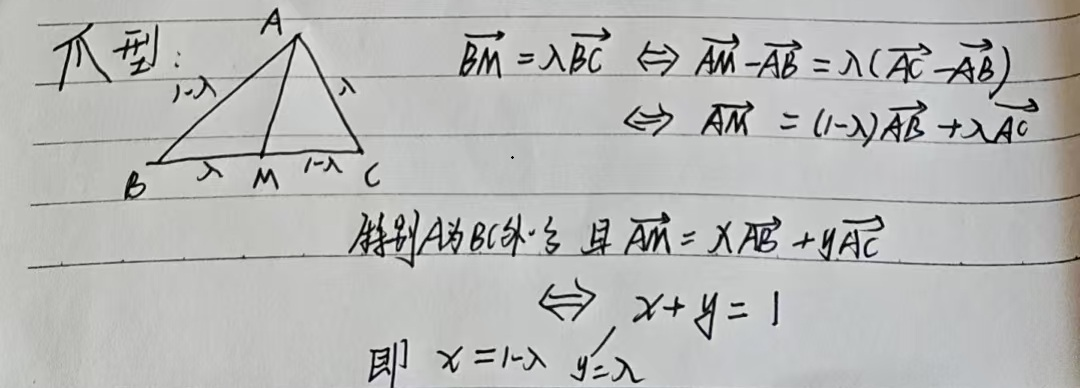
\includegraphics[width=\linewidth]{“爪”型}
	\end{center}
	
\end{liti}

	
\end{document}